
Here we present our results for the full cluster rate and for two
galaxy subsets (\S\ref{sec:clrate_results_results}) and summarize
contributions to the uncertainty (\S\ref{sec:clrate_results_sys}) in
each. In \S\ref{sec:ratevscut} we show that the rate result in the subsets
are not sensitive to the specific parameters used to select the
subset.

\subsection{Results} \label{sec:clrate_results_results}

%%%%%%%%%%%%%%%%%%%%%%%%
% TABLE: CLUSTER RATES %
%%%%%%%%%%%%%%%%%%%%%%%%
\begin{table}
\caption{\label{tab:clrates}Results: cluster SN~Ia rate}
\begin{center}
\begin{footnotesizetabular}{lccccccc}
\hline
\hline
Environment & Unit & $\bar{z}$ & $N_{\rm SN~Ia}$ & Denom & Rate & (stat) & (sys) \\
\hline
Full cluster & SNuB & 1.14 & $8.0 \pm 1.0$ & 15.87 & 0.50 & $^{+0.23}_{-0.19}$ & $^{+0.10}_{-0.09}$\\
Full cluster & SNug & \nodata & \nodata & 15.96 & 0.50 & $^{+0.23}_{-0.19}$ & $^{+0.10}_{-0.09}$\\
Full cluster & SNuM & \nodata & \nodata & 22.41 & 0.36 & $^{+0.16}_{-0.13}$ & $^{+0.07}_{-0.07}$\\
Red-sequence & SNuB & 1.13 & $6.5 \pm 0.5$ & 11.95 & 0.54 & $^{+0.25}_{-0.19}$ & $^{+0.07}_{-0.07}$\\
Red-sequence & SNug & \nodata & \nodata & 12.20 & 0.53 & $^{+0.24}_{-0.19}$ & $^{+0.07}_{-0.07}$\\
Red-sequence & SNuM & \nodata & \nodata & 17.61 & 0.37 & $^{+0.17}_{-0.13}$ & $^{+0.05}_{-0.05}$\\
Red-sequence early-type & SNuB & 1.10 & $6.0 \pm 0.0$ &  7.29 & 0.82 & $^{+0.39}_{-0.30}$ & $^{+0.09}_{-0.08}$\\
Red-sequence early-type & SNug & \nodata & \nodata &  7.59 & 0.79 & $^{+0.38}_{-0.29}$ & $^{+0.09}_{-0.08}$\\
Red-sequence early-type & SNuM & \nodata & \nodata & 11.77 & 0.51 & $^{+0.24}_{-0.19}$ & $^{+0.06}_{-0.05}$\\
\hline
\end{footnotesizetabular}

\end{center}
{\footnotesize
{\bf Note.} --- ``Denom'' is the denominator of
equation~(\ref{eq:rate}) and has units of $10^{12} L_{\odot,B}$~years,
$10^{12} L_{\odot,g}$~years and $10^{12} M_\odot$~years for rate units
of SNuB, SNug and SNuM respectively.}
\end{table}

The results are presented in Table~\ref{tab:clrates}.  We derive a
rate in the full cluster, in red-sequence galaxies only, and in
red-sequence early-type galaxies only. Each subset includes a
different number of SNe: We have discovered $8 \pm 1$ cluster SNe,
where the quoted uncertainty is due to classification uncertainty
(including uncertainty in both SN type and cluster membership).
Limiting the sample to only SNe discovered in galaxies included in the
red-sequence subset excludes SN~SCP06F12 and SN~SCP06C1, leaving
$6.5 \pm 0.5$ cluster SNe~Ia. The uncertainty here comes from the
uncertainty in the cluster membership and type of SN~SCP06E12, which
we count $0.5 \pm 0.5$ cluster SNe~Ia.  Further limiting the sample to
only SNe discovered in galaxies included in the red-sequence
early-type subset, SN~SCP06E12 is eliminated as its host galaxy is
dimmer than the $z_{850} = 24$ cutoff used for this subset leaving $6$
SNe~Ia with negligible classification error. The number of SNe~Ia
discovered in each subset, including classification error, is
summarized in Table~\ref{tab:clrates} under $N_{\rm SN~Ia}$.

We normalize the rate in three different ways: by $B$-band luminosity,
by $g$-band luminosity, and by stellar mass.  For each cluster, we use
the visibility time map $T(x,y)$ (e.g., Fig.~\ref{fig:ctmaps}) and the
measured luminosity (or mass) profile to carry out the integral in
equation~(\ref{eq:ratedenom}) giving the time-luminosity searched. The
sum of these values for all 25 clusters is the denominator of
equation~(\ref{eq:rate}), the total time-luminosity searched in all
clusters. This is shown in Table~\ref{tab:clrates} under ``Denom''
for each sample. The rate is simply $N_{\rm SN~Ia}$ divided by
``denom,'' as in equation~(\ref{eq:rate}). The contributions to the
statistical and systematic errors are summarized in
Table~\ref{tab:clrate_sys}.

The weighted-average redshift, $\bar{z}$, for each subsample is given by
\begin{equation}
\bar{z} = \frac{\sum_i z_i \int_{x,y} T_i(x,y) L_i (x,y)}
        {\sum_i \int_{x,y} T_i (x,y) L_i (x,y)},
\end{equation}
where $z_i$, $L_i$ and $T_i$ are the redshift, luminosity and
effective visibility time of the $i$-th cluster, respectively. The
weighted-average redshift is slightly smaller for the red-sequence and
red-sequence early-type galaxy subsets. This is because in the
higher-redshift clusters, a smaller fraction of galaxies meet the
subset requirements (see $z<1.2$ versus $z>1.2$ average cluster
luminosity in Table~\ref{tab:lum_avg}).


\subsection{Summary of Systematic Uncertainties} \label{sec:clrate_results_sys}

\begin{table}
\caption{\label{tab:clrate_sys}Sources of uncertainty in cluster SN~Ia rate}
\begin{center}
\begin{footnotesizetabular}{l c c c}
\hline
\hline
                &  Full    &   Red-    & Red-sequence \\ 
                & cluster  & sequence  & early-type   \\
Source of error &  (\%)    &   (\%)    &     (\%)     \\
\hline
\hline
\multicolumn{4}{c}{Statistical} \\
\hline
Poisson                 & $^{+40}_{-32}$ & $^{+45}_{-35}$ & $^{+47}_{-36}$\\
Luminosity (stat)       & $\pm 12$      & $\pm 6$       & $\pm 6$     \\
Luminosity (cosmic var.)& $\pm 16$      & $\pm 4$       & $\pm 3$     \\[0.1in]
\bf{Total statistical}  & $^{+45}_{-38}$ & $^{+46}_{-35}$ & $^{+48}_{-37}$\\[0.1in]
\hline
\multicolumn{4}{c}{Systematic} \\
\hline
SN type classification  & $\pm 13$      & $\pm 8$       & \nodata    \\
Control time: varying $M_B$& $^{+8}_{-6}$   & $^{+8}_{-6}$& $^{+8}_{-6}$ \\
Control time: dust distribution & $^{+10}_{-2}$ & \nodata & \nodata     \\
Luminosity: MAG\_AUTO corr.    & $\pm 7$       & $\pm 7$   & $\pm 7$\\
Luminosity: $K$-correction          & $\pm 3$       & $\pm 3$   & $\pm 3$\\
Luminosity: Faint galaxy corr. & $^{+4}_{-9}$   & \nodata   & \nodata\\
Luminosity: $r>0.6$(0.8)~Mpc  & $\pm 4$   & $\pm 1$    & $\pm 1$\\[0.1in]
\bf{Total systematic} & $^{+20}_{-19}$ & $^{+14}_{-12}$  & $^{+11}_{-10}$\\[0.1in]
\hline 

\bf{Total statistical $+$ systematic} & $^{+49}_{-42}$ & $^{+48}_{-37}$ & $^{+49}_{-38}$ \\
\hline
\end{footnotesizetabular}
\end{center}
\end{table}

Throughout the paper, we have highlighted and addressed possible
sources of systematic uncertainty. Here we summarize these sources.
In Table~\ref{tab:clrate_sys} we show the relative contribution of
each to the total systematic error, and compare to sources of
statistical error.

(1) \emph{SN type classification:} The uncertainty in the number of
SNe observed in each galaxy subset was addressed in
\S\ref{sec:clrate_results_results}. The fractional error in the rate is simply the
fractional error in the number observed.

(2) \emph{Control time: Varying $M_B$:} In our control time
simulations, we assumed a distribution of SN~Ia light curve shapes and
absolute magnitudes. To first order, the impact of these assumptions
on the control time is captured by varying the assumed SN~Ia absolute
magnitude (\S\ref{sec:ct_sys}). Variations of $\pm 0.2$~mag resulted in a
rate change of $^{+8}_{-6}\%$

(3) \emph{Control time: dust distribution:} In \S\ref{sec:ct_sys} we
assessed the impact of varying amounts of dust extinction on the
control time. Assuming an unrealistically large amount of
dust-affected SNe decreased the control time by 9\% (increasing the SN
rate by $10\%$), while decreasing the amount of dust-affected SNe
increased the control time by $2\%$ (decreasing the SN rate by
$2\%$). We do not apply this systematic error to the red-sequence or
red-sequence early-type subsets, as we have independent evidence that
the amount of dust is limited in these environments.

(4) \emph{MAG\_AUTO correction:} In computing the total $z_{850}$ luminosity
of each galaxy, we made a correction to the MAG\_AUTO magnitude
ranging from $\sim$10\% at $z_{850}=20$ to $\sim$30\% at
$z_{850}=25$. Varying the range of $n$ used in the simulation by $\pm
1$ affects the correction by $\pm 7\%$.

(5) \emph{$K$-correction:} In \S\ref{sec:lum_kcorr}, we noted that the
scatter of BC03 templates about the best-fit $K$-correction is
typically less than 0.03~mag. We use this value as the systematic
error on the $K$-correction.

(6) \emph{Faint galaxy correction:} The average correction $C$
reported in Table~\ref{tab:lum_params} is 1.054. Varying $M^\ast_B$ by
$\pm$ 0.5~magnitudes results in an average correction of 1.032 and
1.092 for $-0.5$ and $+0.5$~magnitudes, respectively. Varying $\alpha$
by $\pm 0.2$ results in an average correction of 1.027 and 1.098 for
$\alpha = -0.7$ and $-1.1$, respectively. Concurrently varying
$M^\ast_B$ and $\alpha$ within the same ranges results in a minimum
average correction of 1.015 ($M^\ast_B = -22.2$, $\alpha = -0.7$) and a
maximum average correction of 1.154 ($M^\ast_B = -21.2$, $\alpha =
-1.1$). Conservatively, we assign $^{+4\%}_{-9\%}$ as the systematic
error on the rate associated with this correction. This error is not
applied to the red-sequence or red-sequence early-type subsets because
these subsets do not include light from galaxies below the detection
threshold.

(7) \emph{Luminosity at large radii:} In \S\ref{sec:lum_profiles} we assumed
a model for the cluster luminosity profile at $r>0.6$~Mpc (0.8~Mpc for
red-sequence and red-sequence early-type subsets). Varying the model
luminosity by $\pm 20\%$ resulted in a $\pm 4\%$ change in the full
cluster rate. The change is much smaller ($\pm 1\%$) for the red
galaxy subsets because the model is only used at $r>0.8$~Mpc.

(8) \emph{$M/L$ ratio:} In \S\ref{sec:lum_mass} we used a $M/L$ ratio to
translate stellar luminosity to stellar mass. Rather than estimating
the absolute uncertainty in the $M/L$ ratio (which is strongly
dependent on assumptions), we estimated the uncertainty in
the \emph{evolution} of the $M/L$ ratio from low to high
redshift. This is the relevant uncertainty for comparing rates at
different redshifts in order to derive the SN~Ia delay time
distribution. We defer discussion of this uncertainty
to \S\ref{conclusionssys} where we discuss uncertainties in the DTD.


\subsection{Effect of Varying Subset Requirements} \label{sec:ratevscut}

In selecting our red-sequence and red-sequence early-type galaxy
subsamples, we required red-sequence galaxies to be within $\pm
0.2$~mag of the color of their cluster red sequence. For early-type
galaxies, we required the asymmetry parameter to be $< 0.1$ and the
Gini coefficient to be $> 0.40$. It is interesting to test the
sensitivity of the results to variations in the requirements. In
Figures~\ref{fig:ratevscut1} and~\ref{fig:ratevscut2} we vary the
requirements and observe the effect on the rates. As requirements are
made more strict (for example, narrowing the red sequence) the total
mass of the sample decreases. At the same time, SNe fall out of the
sample when their host galaxies are cut. The Poisson error increases
as the number of included SNe shrinks.

%%%%%%%%%%%%%%%%%%%%%%%%%%%%%%%%%%%%%
% PLOTS: Rate vs cut                %
%%%%%%%%%%%%%%%%%%%%%%%%%%%%%%%%%%%%%

\begin{SCfigure}[1.][tbh]
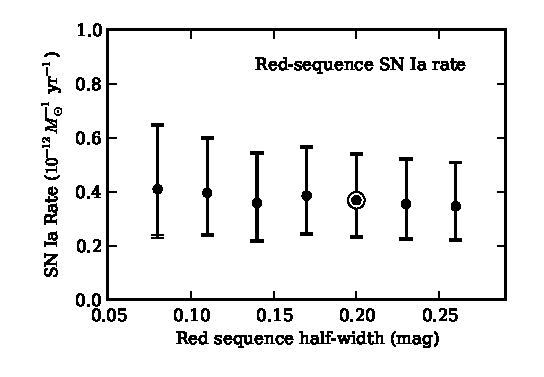
\includegraphics[width=0.6\textwidth]{figures/clrate/ratevscut1.eps}
\caption[Red-sequence-only rate versus width of red sequence]
{The effect of varying the width of the red sequence on the
  red-sequence-only rate. The nominal red-sequence rate result
  corresponds to a half-width of 0.20~mag. The inner and outer error
  bars represent the statistical and total uncertainty, respectively.
\label{fig:ratevscut1}}
\end{SCfigure}

\begin{SCfigure}[1.][tbh]
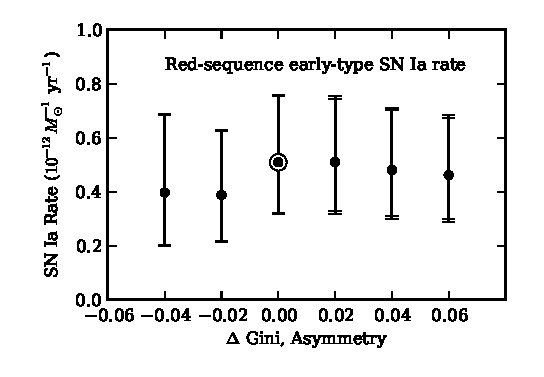
\includegraphics[width=0.6\textwidth]{figures/clrate/ratevscut2.eps}
\caption[Elliptical-only rate versus morphology requirements]
{The effect of varying the morphology parameter requirements. Negative
  $\Delta$ values correspond to a more strict selection and a
  higher-purity early-type galaxy sample. The requirements are
  asymmetry $<0.1+\Delta$ and Gini coefficient $> 0.40-\Delta$. The
  nominal red-sequence early-type rate corresponds to $\Delta = 0$.
  The red-sequence half-width is fixed at 0.2~mag. The inner and outer
  error bars represent the statistical and total uncertainty,
  respectively.
\label{fig:ratevscut2}}
\end{SCfigure}


There is not a strong dependence of the SN~Ia rate with galaxy color
residual from the red sequence (Fig.~\ref{fig:ratevscut1}). Even in
cluster galaxies that lie in a tight range around the red-sequence
($\pm 0.08$~mag), we find a SN~Ia rate consistent with the full
cluster rate. Similarly, there is no significant rate trend with the
purity of the early-type sample (Fig.~\ref{fig:ratevscut2}). We
happened to pick morphology requirements that yield a slightly higher
rate than other choices, but such variations are expected with
small-number statistics and are accounted for by the Poisson
uncertainty in the result (Tables~\ref{tab:clrates}
and~\ref{tab:clrate_sys}). Even in the most-selective subset ($\Delta
= -0.04$), the rate is consistent with the full cluster rate.
